% arXiv submission source.
%
% Compiles with pdflatex (arXiv's default). Deliberately conservative:
%   - only packages shipped with TeX Live;
%   - no \pdfoutput (arXiv forbids forcing the output format);
%   - no external figure files - Figure 1 is pgfplots source, so nothing
%     needs converting and no JPEG/PNG/PDF asset has to travel with it;
%   - bibliography inlined as thebibliography, so there is no .bib/.bbl
%     name-matching to get wrong;
%   - single directory, no subdirectories;
%   - no line numbers, watermarks or margin notes (arXiv rejects these).
\documentclass[11pt]{article}

\usepackage[T1]{fontenc}
\usepackage[utf8]{inputenc}
\usepackage[margin=1in]{geometry}
\usepackage{amsmath}
\usepackage{booktabs}
\usepackage{graphicx}
\usepackage{pgfplots}
\pgfplotsset{compat=1.17}
\usepackage[hidelinks]{hyperref}
\usepackage{microtype}

\title{What Actually Matters in Road-Level Crash Prediction:\\
Eleven Findings, Four Replications}
\author{Maurya Patel\\\small University of Westminster\\\small \texttt{patelmaurya1112@gmail.com}}
\date{\today}

\begin{document}
\maketitle

\begin{abstract}
We attempt to replicate and extend the STZITD-GNN of Gao et al.\ (2024)
for road-level crash prediction on three London boroughs, using
independently constructed data. Our model reaches AccHR@20 of
$80.08\% \pm 2.62$ (5 seeds) against their reported $72.60\%$,
significantly better on two of three boroughs. But the more transferable
results are negative and methodological: of eleven findings that appeared
significant on a single borough, only four survived replication on a
second. Effect size predicts non-replication but not replication: every
effect below the measured $\sim$4-point seed-noise band failed (4/4),
while only 4 of 6 effects above it survived. Failure is characteristically
a sign reversal rather than a shrinkage toward zero, and one effect
reverses sign between random seeds within a single borough. We further
show that at matched history depth our graph neural network is
statistically indistinguishable from sorting road segments by their past
crash count, and that the reference architecture, given the same data and
its own tuned settings, loses to that sort on 18 of 18 held-out windows
($-17.37$ points, $p < 10^{-6}$, 5 seeds). The sort converts three further
years of history into a significant $+2.95$-point gain ($p = 0.041$) where
the same extension moves our network by $-0.12$ ($p = 0.86$). The
reference paper does include a historical-average baseline, but its data
covers a single year; we argue that the apparent margin of graph networks
over historical baselines in this literature is substantially a function
of how short a horizon those baselines were computed over.
\end{abstract}

\section{What we set out to do, and what we found instead}

The intended contribution was a benchmark improvement. The durable
contribution is an account of how easily results at this evaluation scale
mislead.

\begin{table}[h]
\centering
\small
\begin{tabular}{lrrrr}
\toprule
Borough & This work & 95\% CI & Gao et al. & \\
\midrule
Westminster & $\mathbf{79.75\% \pm 0.89}$ & [78.64, 80.86] & 68.98\% & $p<0.0001$ \\
Tower Hamlets & $\mathbf{82.75\% \pm 2.13}$ & [80.11, 85.40] & 72.24\% & $p=0.0004$ \\
Lambeth & $77.75\% \pm 1.67$ & [75.68, 79.82] & 76.59\% & tie, $p=0.1941$ \\
\midrule
\textbf{Pooled} & $\mathbf{80.08\% \pm 2.62}$ & [78.64, 81.53] & 72.60\% & $p<0.0001$ \\
\bottomrule
\end{tabular}
\caption{AccHR@20 over 6 walk-forward windows per borough, averaged over
5 random seeds. $\pm$ is the sample standard deviation; intervals use the
$t$ distribution ($n=5$, $t(4)=2.776$), not the normal approximation,
which would understate them by roughly 40\%.}
\end{table}

\textbf{This is not a like-for-like comparison} and should not be read as
one. Gao et al.\ evaluate within 2019 on a 6:2:2 split; we use multi-year
expanding walk-forward over 2022--2024. No paired test against them is
possible: they publish three point estimates, not per-window results. Our
target is also measurably sparser than theirs (99.97\% zero against their
reported 95.72--96.71\%), a discrepancy we could not resolve after
checking their TCR formula, segment consolidation and evaluation protocol.

\section{Related work}

\textbf{Deep learning for road-level crash prediction.} Gao et
al.~\cite{gao2024} introduce STZITD-GNN, a GAT+GRU encoder with a
zero-inflated Tweedie decoder, evaluated on three London boroughs with
2019 STATS19 data; it is the method we replicate. Nippani et
al.~\cite{nippani2023} assemble the largest benchmark in this line --- 9
million US crash records with road networks and traffic volume --- and
find GraphSAGE predicts monthly counts to within 22\% MAE.

\textbf{Both treat past crashes as the label, not as an input.} Nippani et
al.'s features are graph-structural (degree, betweenness centrality),
weather and traffic volume, and their leave-one-out ablation covers
exactly those three categories: $-6.9\%$, $-2.3\%$ and $-1.2\%$
respectively. Historical crash counts appear as edge \emph{labels} to be
predicted, split temporally, not as a feature the model reads. Gao et al.\
do include a Historical Average baseline, but their dataset covers a
single year, so its horizon is bounded at one.

\textbf{Traditional road safety has used multi-year history for decades.}
The Highway Safety Manual's Empirical Bayes method~\cite{hsm2010} shrinks
an observed count toward a covariate-predicted mean, and is conventionally
applied to three to five years of crash records precisely because shorter
windows are too noisy at site level. That method is a standard baseline in
the practitioner literature and an uncommon one in the deep-learning
literature.

\textbf{The gap this paper addresses} is therefore not a modelling one.
Both communities know that past crashes predict future crashes; the deep
learning line largely encodes that knowledge in the \emph{label} while the
safety-engineering line encodes it in a \emph{multi-year feature}.
Section~\ref{sec:horizon} shows the choice is worth up to 61 points of
AccHR@20 --- more than any architectural difference we measured.

\section{Data and method}

\textbf{Road network.} OS Open Roads (Ordnance Survey, Open Government
Licence), clipped to each borough's administrative \emph{polygon} by an
endpoint-inside test rather than a bounding box --- Westminster's bounding
box extends across the Thames and admits roughly twice the true link
count. Segments are junction-to-junction links; a line-graph transform
gives segment adjacency for message passing. Westminster yields 11,098
directed edges over 4,026 nodes.

\textbf{Target.} Daily collision counts per segment from STATS19 (UK
Department for Transport), 2021--2024, snapped to the nearest edge (median
2.3\,m; 0.22\% beyond 100\,m). The target is 99.97\% zero at segment-day
resolution. We use plain counts rather than a severity-weighted rate; the
weighted variant was tested and is null.

\textbf{Features (35).} Segment geometry and node degree; day of week;
crash history over 7/14/30/90/365 days and 2/3/5 years; casualty-type
breakdown; AADF traffic counts; four OpenStreetMap POI-density classes;
and nine IMD-2019 socio-demographic columns. The long horizons are
computed from the sparse collision list via a cumulative-sum matrix rather
than by rolling over the segment-day table, which would need $\sim$30M
additional rows; this makes horizon length essentially free and is what
allowed the sweep in Section~\ref{sec:horizon}. Features are $z$-scored
with statistics fitted on training instances only.

\textbf{Model.} A GAT layer per timestep feeds a GRU over the resulting
embeddings (3 attention heads, 1 GAT layer, hidden 16/32, residual
connections), decoded by a zero-inflated Poisson head. Adam, learning rate
0.01, 200 epochs, no weight decay or early stopping. Prediction intervals
come from split conformal calibration at 90\% on the last training
instance.

\textbf{Evaluation.} Expanding-window walk-forward: 20-day input, 14-day
horizon, stride 90, six held-out windows per borough spanning 2023-07-15
to 2024-10-07, with training data growing from 6 to 11 instances. The
feature table begins a year before the instance grid so the 365-day
feature is complete for every instance; the grid anchor is
assertion-enforced, because shifting it by the 5-day remainder of
$365 \bmod 90$ would make paired tests match \emph{zero} windows while
still printing plausible output.

\textbf{Metric.} AccHR@20 --- for each day, the share of that day's
crashes falling on the top 20\% of predicted-risk segments, averaged over
the window's days. This is the reference paper's Acc@20.

\textbf{Statistics.} All model figures are means over 5 random seeds
(42, 1, 7, 123, 2024). Comparisons are paired window-by-window and report
both a paired $t$-test and a Wilcoxon signed-rank test; where both arms
are model runs they are paired on seed as well as window, so that a seed's
shared bias cancels.

\section{The main result: replication is the exception}

\begin{table}[h]
\centering
\small
\begin{tabular}{lrl}
\toprule
Finding & Effect (borough 1) & Second borough \\
\midrule
Message-passing depth (1$\to$2 layers) & $-26.46$ & \textbf{replicated} \\
Encoder ordering & $-13.61$ & \textbf{replicated} ($+15.79$ at 5 seeds) \\
Long-horizon crash history & $+15.85$ & \textbf{replicated} ($+9.70$) \\
Our architecture vs.\ theirs & $+18.53$ & \textbf{replicated} ($+13.51$ pooled, 5 seeds) \\
hidden $=42/42$ & $+1.46$ & failed ($-9.97$) \\
Architecture ensembling & $+1.79$ & failed ($p=0.55$, $n=18$) \\
Weight decay $=0.01$ & $+2.53$ & failed ($-0.60$, $n=18$) \\
Road class harmful & $-6.87$ & failed (sign flips, $+2.25$) \\
13 features $\approx$ 35 features & $-0.99$ & failed ($-4.08$, then $+0.77$) \\
Architecture $\times$ history interaction & $+25.04$ & failed (reverses sign) \\
Rank-transform scaling & $+5.80$ & failed ($-39.7$) \\
\bottomrule
\end{tabular}
\caption{Four of eleven survived; seven failed.}
\end{table}

Effect size is often proposed as a filter for which single-sample results
to trust. On this evidence it works in \emph{one direction only}: every
sub-noise effect failed (0 of 4 replicated), so a small effect is reliable
evidence \emph{against} replication --- but two comfortably supra-noise
main effects failed anyway, so a large effect is only weak evidence
\emph{for} it. Road class ($-6.87$, $p=0.016$) reversed sign on the second
borough, and rank-transform scaling went from the best result we recorded
($+5.80$) to the worst ($-39.7$).

\textbf{How failures look matters more than how often they happen.} Four
of the seven were sign reversals, not attenuations. A practitioner who
assumed effects merely shrink across regions --- and therefore treated a
single-region estimate as an upper bound --- would have had the direction
wrong, not just the magnitude.

\section{The model adds little over a trivial baseline}

\begin{table}[h]
\centering
\small
\begin{tabular}{lrrrr}
\toprule
Ranker & Lambeth & Westminster & Tower Hamlets & Mean \\
\midrule
Sort by cumulative crash count ($\sim$8yr) & 83.20\% & 81.25\% & 87.37\% & \textbf{83.94\%} \\
Empirical Bayes (HSM) & 82.11\% & 81.93\% & 87.48\% & 83.84\% \\
Same count, capped to the GNN's 5yr & 80.81\% & 76.46\% & 85.69\% & 80.99\% \\
\textbf{Our GNN} & 77.75\% & 79.75\% & 82.75\% & \textbf{80.08\%} \\
Reference architecture (5 seeds) & --- & --- & --- & 66.57\% \\
\bottomrule
\end{tabular}
\end{table}

Paired window-by-window over the same 18 held-out windows, with the GNN
seed-averaged: at matched history depth the GNN and a parameter-free sort
are statistically indistinguishable ($-0.90$, $p = 0.61$, 9 of 18
windows). Uncapped, both trivial baselines beat it significantly
(Empirical Bayes $-3.76$, $p=0.012$; raw count $-3.85$, $p=0.023$).

\textbf{This is not a property of our implementation alone.} Running the
reference architecture on our data --- at its own swept optimum, with the
same long history, averaged over 5 seeds --- it loses to the crash-count
sort by 17.37 points on \emph{18 of 18} windows ($p < 10^{-6}$), and by
14.41 against the horizon-matched sort. Neither graph network in this
study clears the trivial baseline.

\textbf{Multi-seeding was necessary and changed the surrounding numbers.}
The reference architecture's seed variance is extreme: per-borough spreads
of 18.2, 20.8 and 35.7 points, against $\sim$4 for ours, with one
Westminster seed scoring 42.58\% --- barely twice random. Its per-borough
advantage over ours was consequently mis-estimated in \emph{both}
directions at a single seed ($+18.53$ published against $+9.55$ true on
Lambeth; $+8.01$ against $+13.57$ on Westminster). Pooled over 90 paired
(seed, window) observations our architecture leads by $+13.51$ points, 81
of 90 windows. The direction of every comparison survived; none of the
magnitudes did.

\subsection{The baseline's strength is almost entirely its horizon}
\label{sec:horizon}

This literature does \emph{not} omit a historical baseline. Gao et al.\
report a Historical Average at 44.96\% against their model's 72.60\% --- a
$\sim$28-point margin that reads as clear evidence for the network.
Reconciling that with our sort's 83.94\% requires only one variable: their
dataset covers 2019 alone, so their historical baseline can look back at
most one year.

\begin{figure*}[t]
\centering
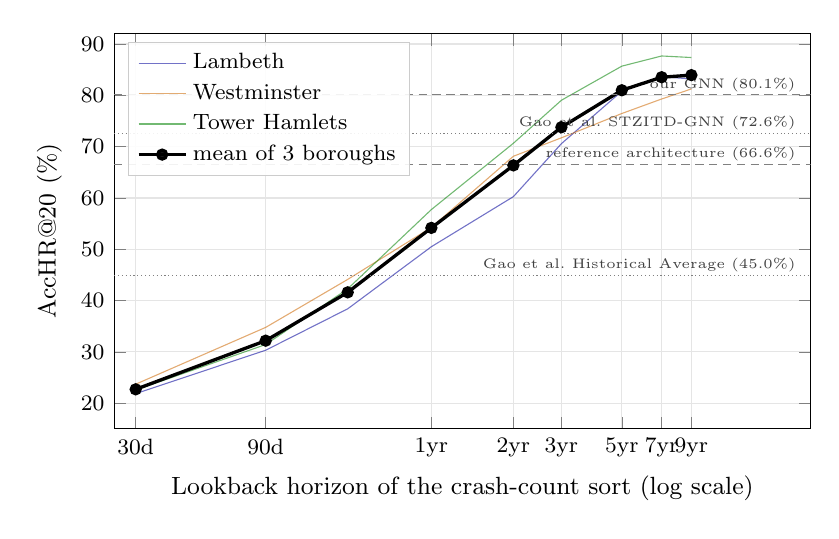
\begin{tikzpicture}
\begin{axis}[
  width=0.86\textwidth, height=6.6cm,
  xmode=log, log basis x=10,
  xlabel={Lookback horizon of the crash-count sort (log scale)},
  ylabel={AccHR@20 (\%)},
  % xmax was 3600 - only 3.9% further out than the last real data point
  % (3285) in LOG space (log10(3600/3285) = 0.039), because a log axis
  % compresses the high end far more than it looks on a linear ruler. The
  % four `anchor=east` reference-line labels below were placed at
  % x=3550, meaning "east" (their text's own right edge) sat there and
  % the text extended LEFTWARD from it - on this axis, a "tiny"-font
  % label's width corresponds to a much wider DATA range at the
  % compressed high end than the same width would at the low end, so
  % every label actually reached back well past x=3285. Three of the
  % four escaped visible collision only because their y-value sits far
  % from the curves' y-range up there (all curves are ~81-87 by 9yr);
  % "our GNN (80.1%)" at y=82.08 does not, and rendered sitting directly
  % on top of the "mean of 3 boroughs" line and its own 9yr marker
  % (confirmed 2026-09-08 by actually compiling this figure with
  % pdflatex for the first time and reading the rendered PDF page - the
  % 39 static structural checks in verify_arxiv_package.py cannot catch
  % a layout collision like this, only a real render can). Fixed at the
  % root rather than nudging one label's y-value: pushed xmax out to
  % 9000 (log10(9000/3285) = 0.437, more than 11x the old log-margin) so
  % there is a genuinely empty region to anchor labels in, and moved
  % every label's anchor to x=8600, safely inside that empty region on
  % this scale.
  xmin=25, xmax=9000, ymin=15, ymax=92,
  xtick={30,90,365,730,1095,1825,2555,3285},
  xticklabels={30d,90d,1yr,2yr,3yr,5yr,7yr,9yr},
  ytick={20,30,40,50,60,70,80,90},
  grid=major, grid style={gray!20},
  tick label style={font=\footnotesize},
  label style={font=\small},
  legend style={font=\footnotesize, at={(0.02,0.98)}, anchor=north west,
                draw=gray!40, fill=white, fill opacity=0.9, text opacity=1},
  legend cell align=left,
]
\addplot[blue!60!black, thin, opacity=0.55, mark=none] coordinates {(30,21.86) (90,30.33) (180,38.40) (365,50.50) (730,60.26) (1095,70.58) (1825,80.81) (2555,83.62) (3285,83.20)};
\addlegendentry{Lambeth}
\addplot[orange!80!black, thin, opacity=0.55, mark=none] coordinates {(30,23.71) (90,34.78) (180,44.13) (365,54.26) (730,68.13) (1095,71.72) (1825,76.46) (2555,79.29) (3285,81.25)};
\addlegendentry{Westminster}
\addplot[green!50!black, thin, opacity=0.55, mark=none] coordinates {(30,22.56) (90,31.44) (180,42.29) (365,57.74) (730,70.66) (1095,79.04) (1825,85.69) (2555,87.67) (3285,87.37)};
\addlegendentry{Tower Hamlets}
\addplot[black, very thick, mark=*, mark size=1.6pt] coordinates {(30,22.71) (90,32.19) (180,41.61) (365,54.17) (730,66.35) (1095,73.78) (1825,80.99) (2555,83.53) (3285,83.94)};
\addlegendentry{mean of 3 boroughs}
\addplot[gray, densely dotted, forget plot] coordinates {(25,44.96) (9000,44.96)};
\node[anchor=east, font=\tiny, gray!50!black] at (axis cs:8600,46.96) {Gao et al.\ Historical Average\ (45.0\%)};
\addplot[gray, densely dashed, forget plot] coordinates {(25,66.57) (9000,66.57)};
\node[anchor=east, font=\tiny, gray!50!black] at (axis cs:8600,68.57) {reference architecture\ (66.6\%)};
\addplot[gray, densely dotted, forget plot] coordinates {(25,72.60) (9000,72.60)};
\node[anchor=east, font=\tiny, gray!50!black] at (axis cs:8600,74.60) {Gao et al.\ STZITD-GNN\ (72.6\%)};
\addplot[gray, densely dashed, forget plot] coordinates {(25,80.08) (9000,80.08)};
\node[anchor=east, font=\tiny, gray!50!black] at (axis cs:8600,82.08) {our GNN\ (80.1\%)};
\end{axis}
\end{tikzpicture}
\caption{The same parameter-free crash-count sort, swept across lookback
horizons on our data and windows. The ranker spans 22.71\% to 83.94\% —
a 61.2-point range — with nothing changing but how far back it looks.
Dashed reference lines are measured on our data; dotted lines are the
reference paper's published figures on theirs, so their vertical position
is indicative rather than a controlled comparison.}
\label{fig:horizon}
\end{figure*}


The same ranker spans 22.71\% to 83.94\% with no change but how far back
it looks. Each published figure is matched by a sort at a strikingly short
horizon: their Historical Average at $\sim$1 year, the reference
architecture at $\sim$2, their model at $\sim$3, ours at $\sim$5. This
mapping is suggestive, not controlled --- two of those figures are on
their data --- but the quantity of published improvement over a historical
baseline in this task is of the same order as the improvement obtainable
by lengthening that baseline's horizon by a year or two, on data freely
available to both. We could find no paper in this line that reports it.

The curve plateaus after about seven years, which corrects an earlier
reading of our own: at three years it is still climbing steeply and
appears not to plateau at all.

\section{Measurement properties practitioners should know}

\begin{itemize}
\item \textbf{Seed variance is large and its sign is borough-specific.}
Spread 3.2--4.7 points across 5 seeds for our architecture. One seed was
$+1.69$ optimistic on one borough and $-1.11$ conservative on another, so
a seed's bias measured on one region cannot correct another.

\item \textbf{The metric is a step function, and its step size is set by
target sparsity.} AccHR@20 averages a per-day hit rate, so its smallest
possible change is one crash crossing the threshold on one day:
$1/(\text{crashes that day})/(\text{days in window})$. On our windows that
is 0.0102--0.0909. Because 94\%+ of segments are tied at zero recent
crashes, a floating-point difference invisible in the predictions can
reorder a tie group and move one crash across the cut. \emph{No AccHR@20
figure on a sparse window should be quoted more precisely than its own
step size.}

\item \textbf{Training is not deterministic at a fixed seed.} Re-training
one window at one seed three times gave 0.755, 0.832 and 0.845 --- a
spread of 9.0 points --- while a control window on another borough was
bit-identical across three repeats. The GAT layer's neighbourhood
aggregation is scatter-based and CUDA does not fix accumulation order;
seeding makes initialisation reproducible but not aggregation. Enabling
deterministic algorithms should be the default for new work on this task.

\item \textbf{The reference paper's architectural choices fail by
divergence, not degradation.} Depth 2 diverges on 2 of 6 Westminster
windows; the full reference architecture spreads 35.7 points across seeds;
their encoder ordering costs $\sim$6 points on four seeds but collapses to
near-random on the fifth, on the same seed in both boroughs. A mean over
seeds misdescribes all three, and the failure rate ($\sim$1 in 5 here) is
the more useful quantity.

\item \textbf{The metric depends on crash volume.} AccHR@20 rises
$\sim$0.39 points per additional crash in a window ($p=0.0316$, $n=31$).

\item \textbf{Holiday periods are genuinely harder}, $-11.14$ points
independent of crash volume ($p=0.0078$).

\item \textbf{Controls pass.} A constant prediction scores 10.12\%, below
random's $\sim$20\%, so no reported score is a tie-breaking artefact; and
permuting targets across segments collapses the model from 75.64\% to
23.08\%.
\end{itemize}

\section{Limitations}

Three boroughs for the benchmark comparison (seven for generalisation);
six windows per borough; one city; and a target-density discrepancy
against the reference paper that we could not explain.

\textbf{Individual figures are less precise than their digits suggest.} We
observed one window take three different values across three independent
runs of the same configuration and seed, separated by exact single-crash
steps, while its five sibling windows were bit-identical. A per-borough
mean over six such windows can shift by roughly 0.3 points between runs
for reasons unrelated to the model. Readers should treat per-borough
numbers as accurate to a few tenths of a point.

\textbf{Generalisation.} Across seven London boroughs at a single seed the
model ranges 73.83--84.66\%, so performance does not collapse outside the
benchmark set. Brent --- the only outer-London borough and the least
POI-dense --- has by far the widest per-window spread, consistent with the
measured dependence of AccHR@20 on crash volume.

\textbf{A data-collection failure worth reporting.} The OSM Overpass API
degraded mid-study, reporting free capacity while truncating larger
transfers. One borough's POI download lost an entire feature category on
four separate attempts while appearing successful. The failure was
silent: it produced a plausible-looking file that would have been cached
and reused indefinitely. When that borough was eventually downloaded
intact, the truncated file proved to have held 24\% of the real data. We
now refuse such responses in code, checking that every category returned
and that POI density clears a floor calibrated on verified downloads.

\section{Reproducibility}

Every quantitative claim above is regenerated by a named script in the
accompanying repository. Two verifiers guard the write-up: one re-derives
each headline number from its source file and compares it against this
document, exiting non-zero on any mismatch; the other checks that the
repository's README, model specification and this paper do not disagree
with one another --- a class of error single-document verification cannot
detect, and which produced two real discrepancies during drafting.

Data: STATS19 (UK Department for Transport), OS Open Roads (Ordnance
Survey, Open Government Licence), IMD 2019, DfT AADF --- all free, none
redistributable here; the repository gives acquisition URLs and target
paths. The full decision log, including every withdrawn claim and the
reasoning behind it, is included.

\begin{thebibliography}{9}

\bibitem{gao2024}
X.~Gao, X.~Jiang, D.~Haworth, D.~Zhuang, S.~Wang, H.~Li, et al.
\newblock Uncertainty-aware probabilistic graph neural networks for
  road-level traffic crash prediction.
\newblock \emph{Accident Analysis \& Prevention}, 208:107801, 2024.

\bibitem{nippani2023}
A.~Nippani, D.~Li, H.~Ju, H.~Koutsopoulos, and H.~R. Zhang.
\newblock Graph neural networks for road safety modeling: Datasets and
  evaluations for accident analysis.
\newblock In \emph{Advances in Neural Information Processing Systems 36
  (NeurIPS 2023) Datasets and Benchmarks Track}, 2023.

\bibitem{hsm2010}
American Association of State Highway and Transportation Officials.
\newblock \emph{Highway Safety Manual}, 1st edition, 2010.

\end{thebibliography}

\end{document}
